\documentclass[11pt, norsk]{article}

\usepackage{kantlipsum}   %% only for demo
\usepackage[utf8x]{inputenc}
\usepackage[T1]{fontenc}
\usepackage{lmodern}
\usepackage{marvosym}
\usepackage{graphicx}

\usepackage[final]{pdfpages}

\pagestyle{empty}

\usepackage[scale=0.775]{geometry}
\setlength{\parindent}{0pt}
\addtolength{\parskip}{6pt}

\def\firstname{Anders}
\def\familyname{Østevik}
\def\FileAuthor{\firstname \familyname}
\def\FileTitle{Søknad inforsentered UiB}
\def\FileSubject{Søknad}
\def\FileKeyWords{\firstname \familyname, Søknad, UIB, infosenteret}

\renewcommand{\ttdefault}{pcr}

\usepackage{url}
\urlstyle{tt}
\ifpdf
  \usepackage[pdftex,pdfborder={0 0 0},breaklinks,baseurl=http://,pdfpagemode=None,pdfstartview=XYZ,pdfstartpage=1]{hyperref}
  \hypersetup{
    pdfauthor   = \FileAuthor,%
    pdftitle    = \FileTitle,%
    pdfsubject  = \FileSubject,%
    pdfkeywords = \FileKeyWords,%
    pdfcreator  = \LaTeX,%
    pdfproducer = \LaTeX}
\else
  \usepackage[dvips]{hyperref}
\fi

\begin{document}
\sffamily   % for use with a résumé using sans serif fonts;
%\rmfamily  % for use with a résumé using serif fonts;
\hfill%
\begin{minipage}[t]{.6\textwidth}
\raggedleft%
{\bfseries Anders Østevik}\\[.35ex]
\small\itshape%
Fantoftveien 14L\\
Postboks 1267, 5075 BERGEN\\[.35ex]
\Telefon~984 92 338\\
\Letter~\href{mailto:anders.ostevik91@gmail.com}{anders.ostevik91@gmail.com}
\end{minipage}\\[1em]
%
\begin{minipage}[t]{.4\textwidth}
\raggedright%
{\bfseries SAIV A/S, Bergen}\\[.35ex]
\small\itshape%
Nygardsviken 1\\
5164 Laksevag
\end{minipage}
\hfill % US style
%\\[1em] % UK style
\begin{minipage}[t]{.4\textwidth}
\raggedleft % US style
\today
%Mai 25, 2016 % US informal style
%25/05/2016 % UK formal style
\end{minipage}\\[2em]
\raggedright

%Søknad om stilling som sommervikar i infosenteret.
%
Søker med dette på stilling som sommervikar i Infosenteret ved Realfagsbygget, Universitetet i Bergen.\\[1.5em]
Jeg er 24 år gammel, samboer, ingen barn. Jeg har fra før utdanning som elektroingeniør med bachelor i elektronikk fra Høgskolen i Bergen. For tiden arbeider jeg med min masteroppgave i fysikk, innen mikroelektronikk, og er ferdig nå til sommeren. Jeg skal fra høsten av begynne på nytt studie innen data og programmering, og er på jakt etter sommerjobb og/eller deltidsjobb i det kommende semester.\\[1.0em]

Fra tidligere har jeg relevant erfaring som resepsjonist ved et legesenter, og synes derfor denne stillingen virker interessant. I min tidligere stilling hadde jeg, sammen med en fast ansatt, ansvar for det administrative arbeidet ved legesenteret. Arbeidet gikk blant annet ut på å organisere timelister, besvare generelle spørsmål fra pasienter og å behandle henvendelser som bestilling av pasienttimer, e-resepter og journalutskrifter. Gjennom mitt arbeid som resepsjonist har jeg lært hvordan en bør forholde seg til mennesker med ulike behov, på en rolig og høflig måte. I tillegg er jeg meget datakyndig, og har god erfaring med generell bruk av PC, ulike programmeringspråk, og selvfølgelig alt av officeprogrammer. Videre er jeg meget lettlært i møte med nye dataprogrammer, og tar alt med et smil. Dette er egenskaper jeg mener kan komme godt med som ansatt i Infosenteret ved Realfagsbygget. \\[1.5em]

%Jeg viser interesse til denne stillingen fordi jeg fra før av har erfaringer fra en lignende stilling, som resepsjonist på et legesenter. Som resepsjonist hadde jeg delansvar sammen med en fast ansatt for det administrative arbeidet ved senteret. Arbeidet gikk blant annet ut på organisering av timelister til legene, behandling av bestillinger som pasienttimer, e-resepter og journalutskrifter, samt besvare generelle spørsmål pasientene måtte komme med. Jeg har ved å jobbe som resepsjonist fått god erfaring i det å jobbe med ulike mennesker med ulike behov. I tillegg til god erfaring innen data og programmering mener jeg dette er erfaring som kan komme godt med som ansatt i Infosenteret ved Realfagsbygget. 

Se gjerne vedlagt cv for mer informasjon.\\[1.5em]

Håper på et positivt svar, og kommer gjerne til intervju.\\[3em]

%Yours sincerely,\\[2em] % if the opening is "Dear Mr(s) Doe,"
Med vennlig hilsen,\\[2em] % if the opening is "Dear Sir or Madam,"
%
%\includegraphics[scale=0.75]{signature_blue}\\
{\bfseries Anders Østevik}\\
%
\vfill%
{\slshape Vedlegg: curriculum vitae{}}

\newpage

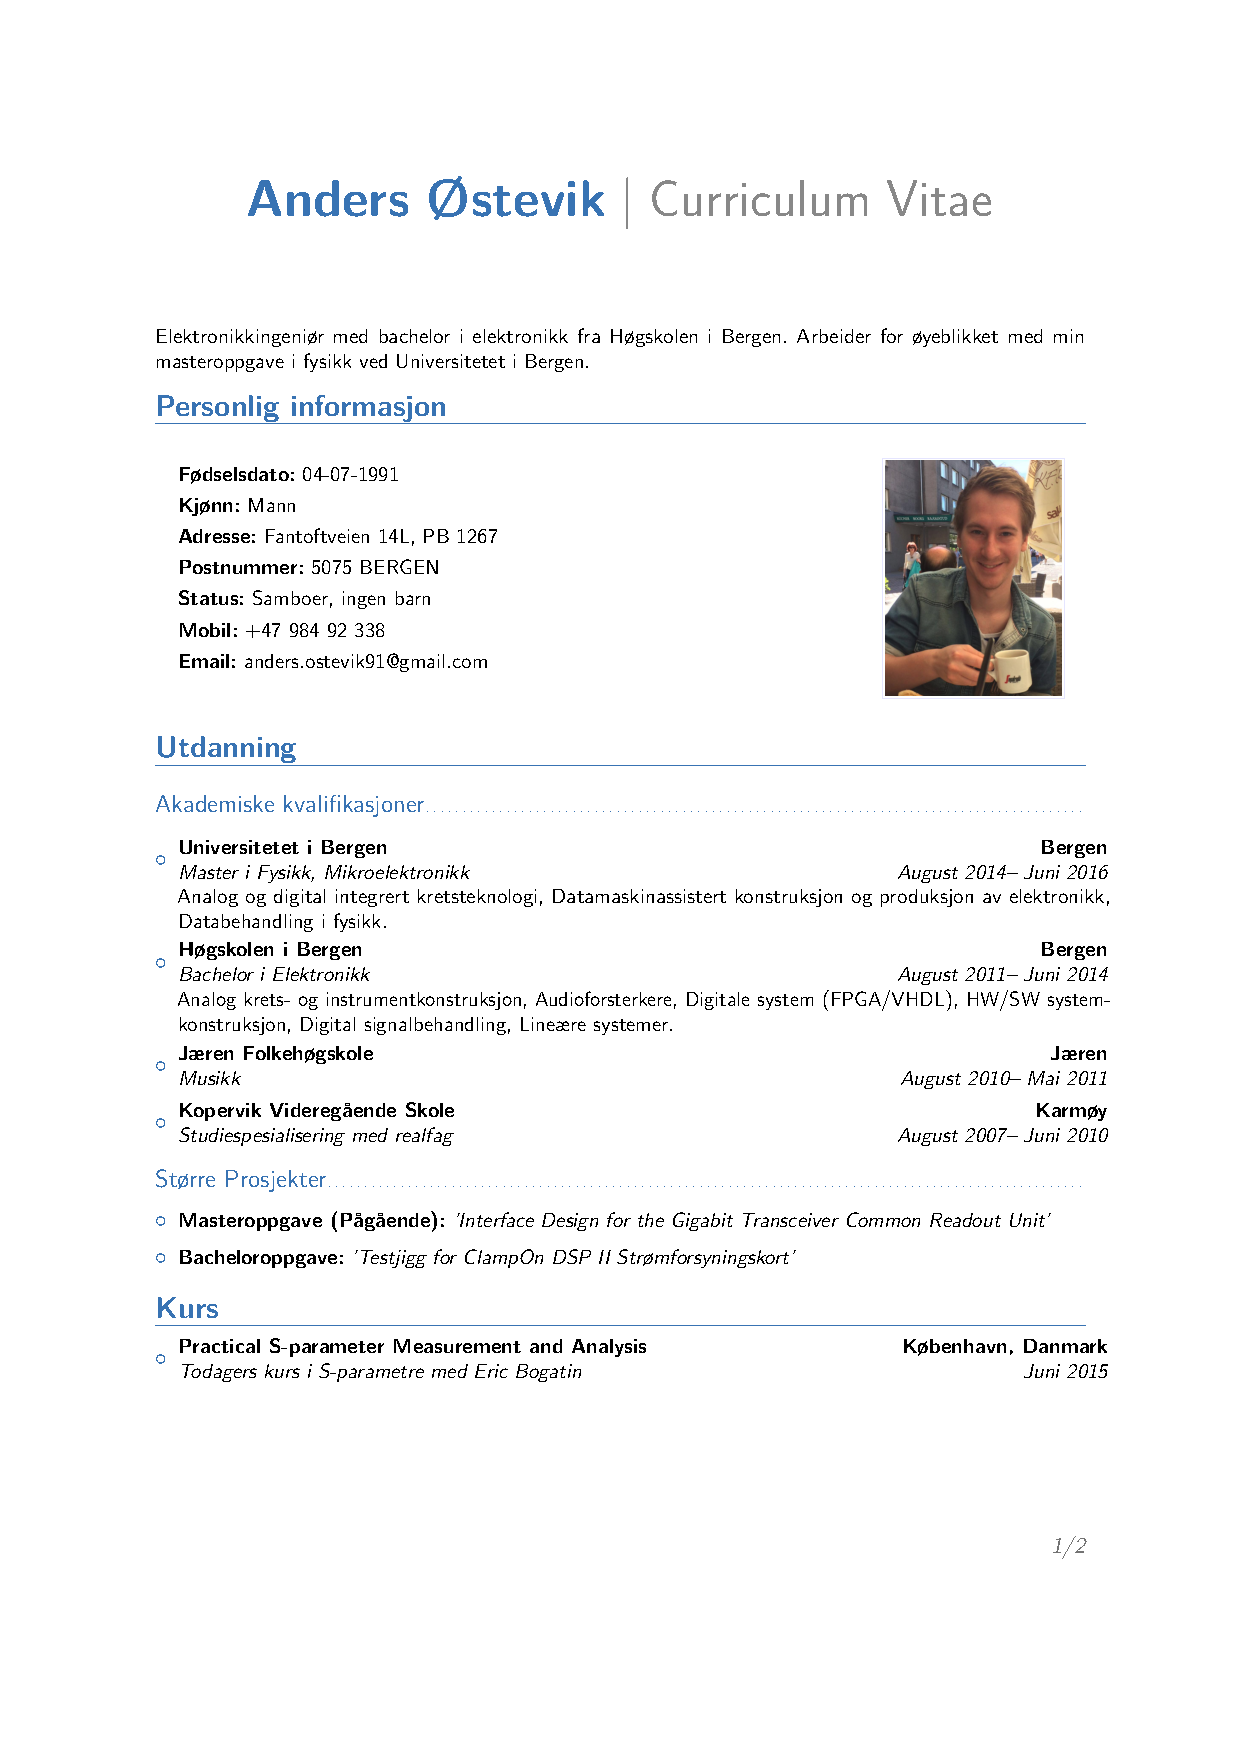
\includepdf[pages=-]{../cv/0602_cv.pdf}

\end{document}